\subsection{Static and Dynamic Kalman Filter - Step on Disturbance}
In this section it is desired to evaluate the performance of the Kalman filter, where a step change occurs in the unknown disturbance. In the previous paragraph, the system was augmented in order to have a proper estimation of the unknown disturbance. This model, is the same used in this paragraph. The consequence of the system not to be augmented, would be that the influence of step change of the disturbance, would move the system away from the linearization point, which is the foundation for the Kalman filter gains. Therefore would the original gains, not be sufficient to drive the difference between the output of the Kalman filter and the true output to be 0. The simulation is carried out as described in the previous paragraph. After 20 minutes, a step change of 10\% occurs in the unknown disturbance.
\begin{figure}[H]
    \centering
    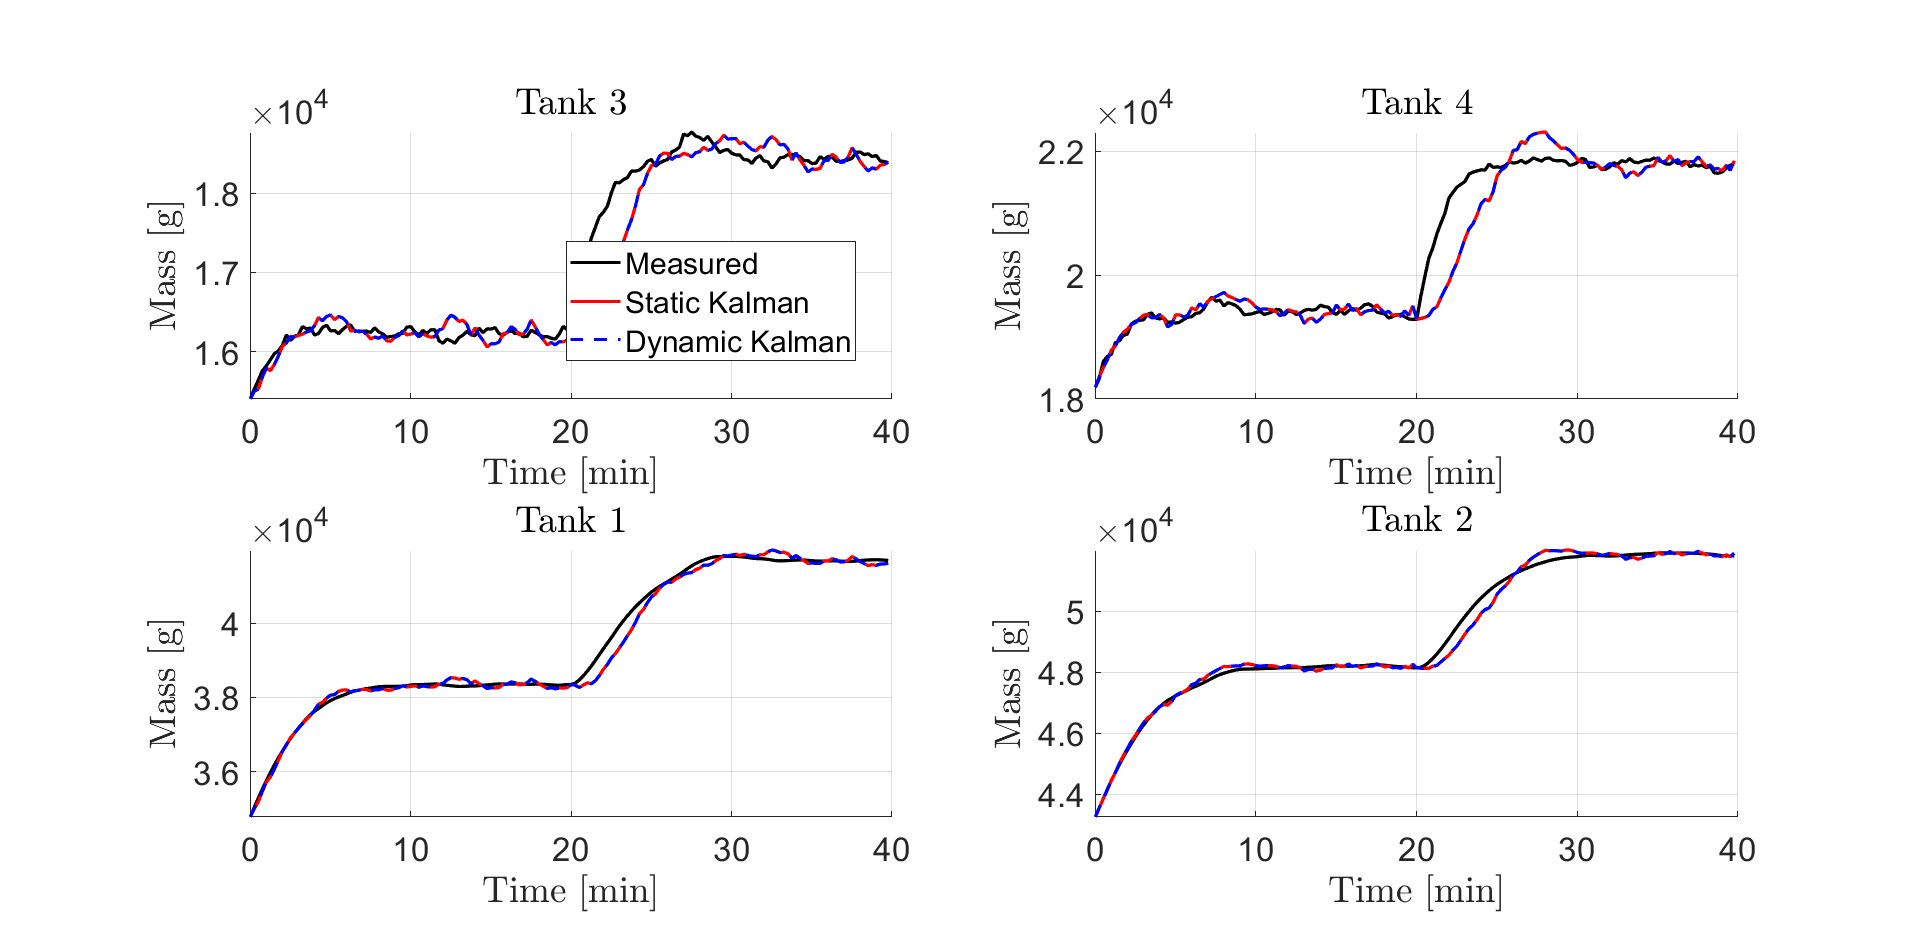
\includegraphics[width=1\textwidth]{Figures/Pr5.3_stoc_states.png}
    \caption{Kalman filter - Stochastic model states}
    %\label{fig:Kalman_stoc_state_step}
\end{figure}
\begin{figure}[H]
    \centering
    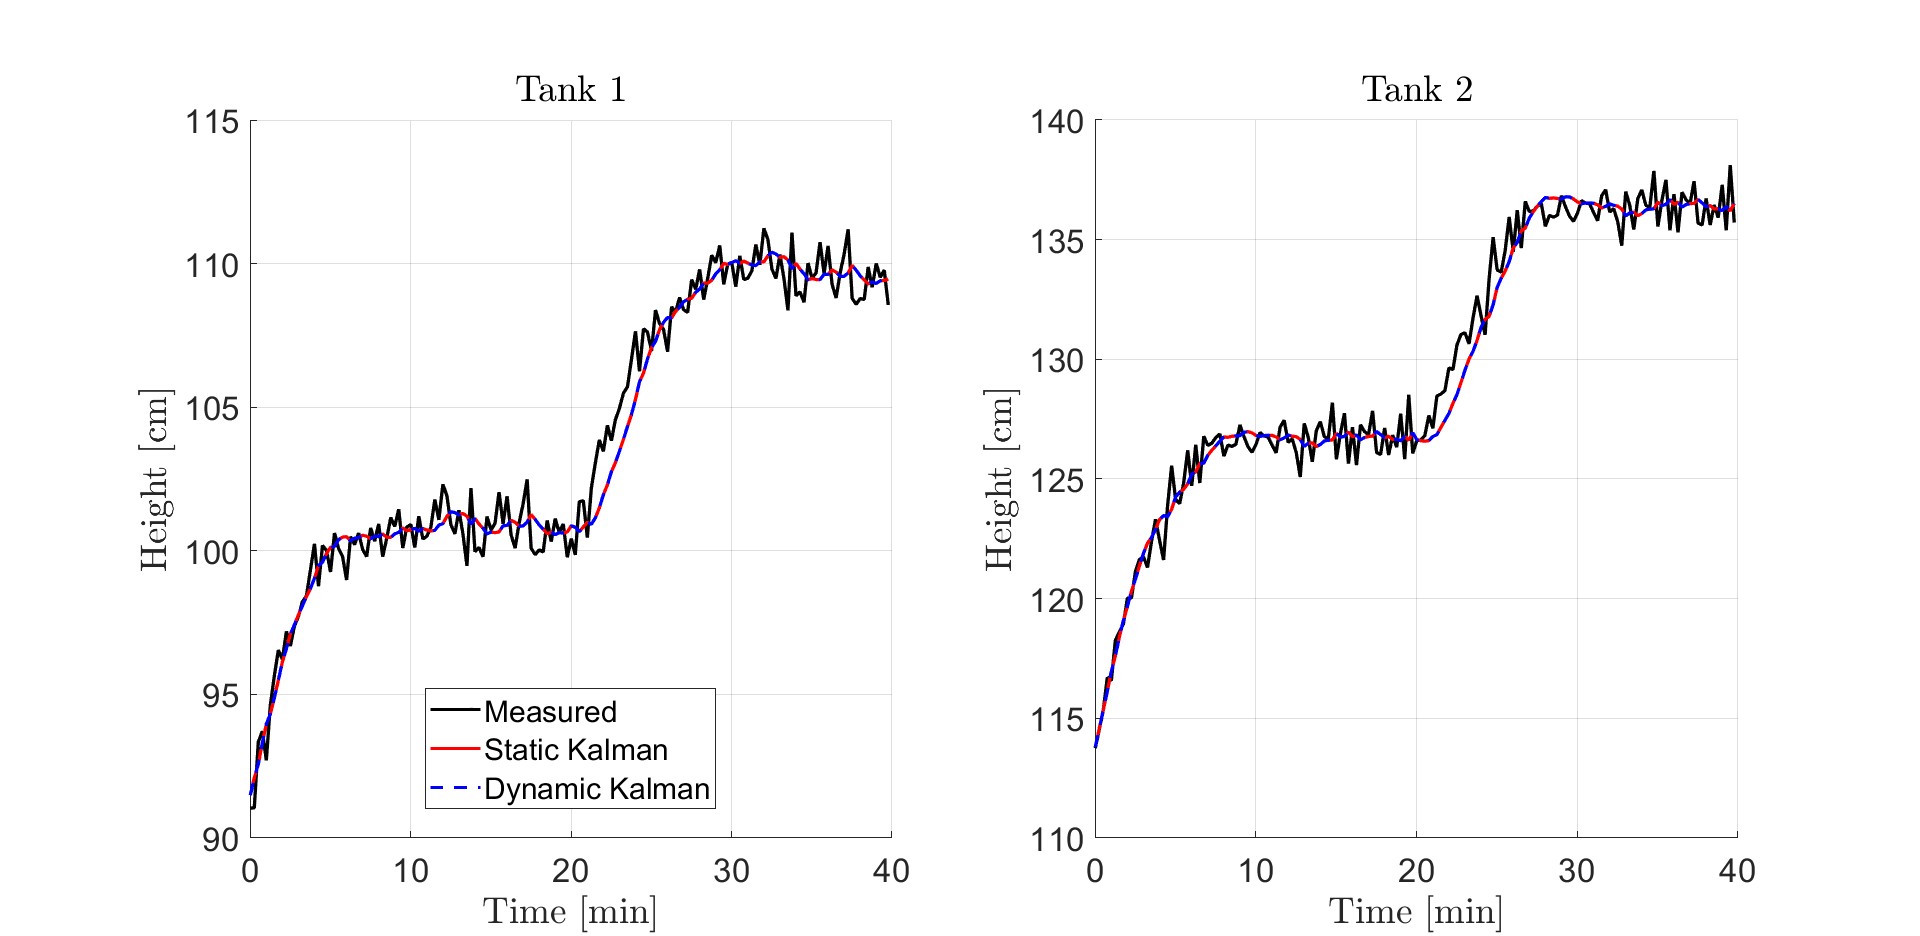
\includegraphics[width=1\textwidth]{Figures/Pr5.3_stoc_output.png}
    \caption{Kalman filter - Stochastic model outputs}
    %\label{fig:Kalman_stoc_state_step}
\end{figure}
It is seen that the Kalman filter is able to estimate the states when the system is perturbed with a step change in the disturbance of 10\%. The Kalman filter also filters the noise as seen on the output. From the estimated states in tank 3 and 4, it can be seen that when a step occurs in the unknown disturbance, there is delay before the Kalman filter is able to adjust the estimate. This is corresponding to the delay from when the step occurs, until the water level raises in tank 1 and 2, so the estimates can use the measurements to adjust.